
\noindent
It was not long ago that bitcoin and the concept of Blockchain appeared for the first time on the Web as a white paper, October 31st 2008 to be more precise “Bitcoin: A Peer-to-Peer Electronic Cash System” \cite{nakamoto_bitcoin_2008} Said the document in its heading. It was uncertain by that time how disruptive such technology could be, and the importance of its role nowadays. A decade later, Bitcoin has consolidated as a strong and reliable asset in which people trust to invest and transfer money. The term “Cryptocurrency” was born. Little after its emission and open source code publication, several teams and individuals started re adapting its code and creating different electronic assets, slowly with its adoption a philosophy more people started trading on their private markets. It would not take too long to foresee the creation of a community and a market craving to trade different assets. As a result of this crescent demand Cryptocurrency market exchanges were created. From the financial perspective, cryptocurrency markets are nowadays allowing people who did not have access to credits or bank accounts before to enter into a different economic world were markets do not sleep, moreover assets can be instantly traded, changed and transferred. Years ago, this market consolidated and matured, data is produced massively, regulations or innovations, even political situations have made the market very peculiar and volatile, something unprecedented in the financial trading.

\begin{figure}[ht]
   \centering
   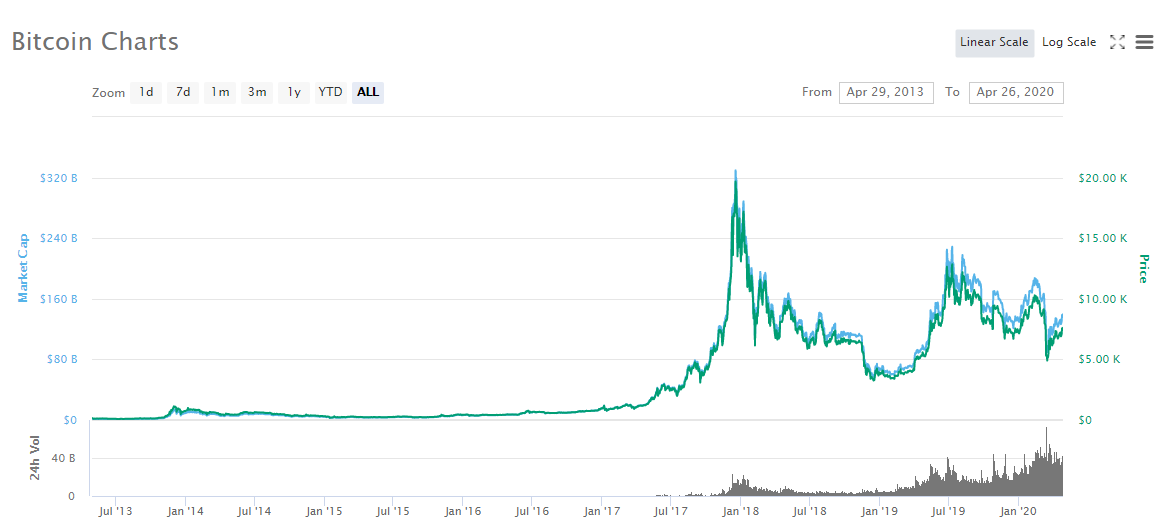
\includegraphics[width=\linewidth]{fig/BitcoinPriceChart.png}
    \caption{Bitcoin price chart (taken from \cite{coinmarketcap_bitcoin_2020})}
    \label{fig:BitcoinChart}
\end{figure}

Bitcoin price volatility generated a high-risk market, but also a lot of interest and market capitalization has been set to the cryptocurrency assets. On April 2020, the total market capitalization of all cryptocurrencies is up to  \$219,165,492,833.00 USD \cite{coinmarketcap_cryptocurrency_2020} which translates in a growing market accessible to anyone with sufficient resources around the world to trade. As the time goes by more resources and assets will be added resulting in an expected increase of profit depending on the investment, but daily fluctuations are visible as well for any asset.

In addition to this, the impact of social media and published news about recent technological progress and Information Technology improvements are expected to be a key player in the decision different traders made to trade cryptocurrency assets. There might be a direct correlation in what is published on social media, news and the price fluctuation of the market in short term basis. It is therefore the aim of this report to explore, discover and predict potential market prices through distributed systems to show the potential of creating a scalable product trained to predict short term prices according to past fluctuations and media publications. 
The system used, algorithms, data set and brief explanation of the challenges in addition to obtain results will be explained in detail though this report. Provided results can be also used as a basis for future work development and algorithm improvements.